% clewin figures, L1 to L5 and alignment marks


\begin{figure}[ht]
    \centering
    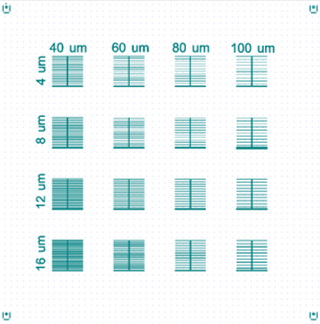
\includegraphics[width=0.45\textwidth]{figures/CleWin_L1.png}
    \caption{
        Layer 1. 
        Numbers on the top is the width of the fingers in the matrix.
        Numbers on the left side is the width of the fingers in the matrix.
        Each LED is 1 mm x 1 mm. 
    }
    \label{fig:CleWin_L1}
\end{figure}


% L2
\begin{figure}[ht]
    \centering
    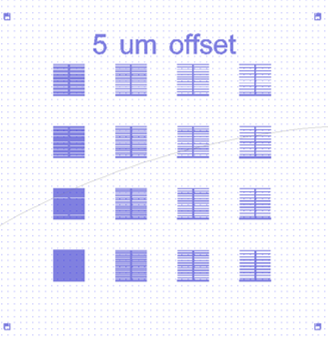
\includegraphics[width=0.45\textwidth]{figures/CleWin_L2.png}
    \caption{
        Layer 2. 
        This is the same as layer 1, but with a 5 \textmu m buffer on the whole pattern. 
    }
    \label{fig:CleWin_L2}
\end{figure}


% L3 
\begin{figure}[ht]
    \centering
    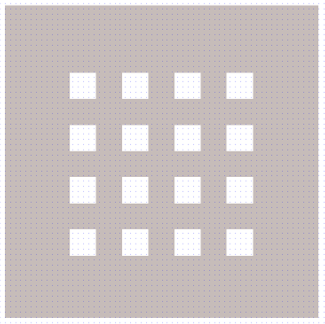
\includegraphics[width=0.45\textwidth]{figures/CleWin_L3.png}
    \caption{
        Layer 3. 
        This is the mesa etch layer. 
        The size of the box covering each LED is 1.012 mm x 1.012 mm.
    }
    \label{fig:CleWin_L3}
\end{figure}

% L4
\begin{figure}[ht]
    \centering
    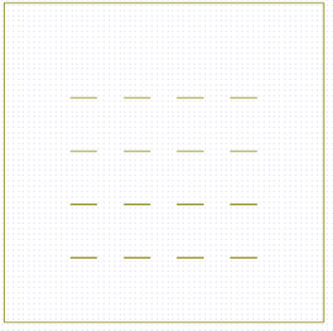
\includegraphics[width=0.45\textwidth]{figures/CleWin_L4.png}
    \caption{
        Layer 4. 
        This is the HF etch layer. 
        Each bar is covering a part of the bottom bus bar, with a size of 20 \textmu m x 980 \textmu m.
    }
    \label{fig:CleWin_L4}
\end{figure}

% L5
\begin{figure}[ht]
    \centering
    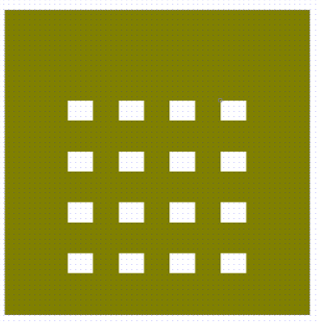
\includegraphics[width=0.45\textwidth]{figures/CleWin_L5.png}
    \caption{
        Layer 5. 
        This is the pad metallization layer, where each box is 1 mm x 0.4 mm. 
        The box is covering the bottom bus bar of each LED. 
    }
    \label{fig:CleWin_L5}
\end{figure}


% Alignment marks
\begin{figure}[ht]
    \centering
    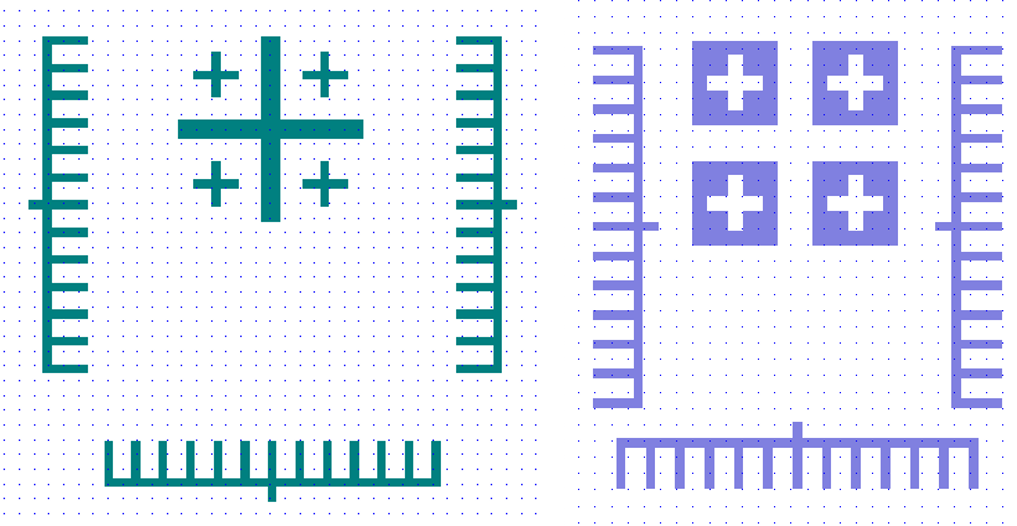
\includegraphics[width=0.45\textwidth]{figures/CleWin_alignment_marks.png}
    \caption{
        Alignment marks for layer 1 and 2. 
        The design allows quantification of the alignment error.
        These marks are the Verniers design. 
    }
    \label{fig:CleWin_alignment_marks}
\end{figure}